\section{Пример: данные об уровне гормона при ношении различных пластырей}

Исторически сложилось так, что статистики очень беспокоились о возможных смещениях в оценках соотношений. Данные об уровне гормона в таблице $10.1$ представляют удобный пример. Восемь субъектов носили медицинские пластыри, предназначенные для введения в кровоток определенного природного гормона. У каждого испытуемого измеряли уровень гормона в крови после ношения трех разных пластырей: пластыря с плацебо, не содержащего гормона, <<старого>> пластыря, произведенного на более старом заводе, и <<нового>> пластыря, произведенного на недавно открывшемся заводе. Первые три столбца таблицы показывают три измерения показателей крови для каждого субъекта.

\noindent
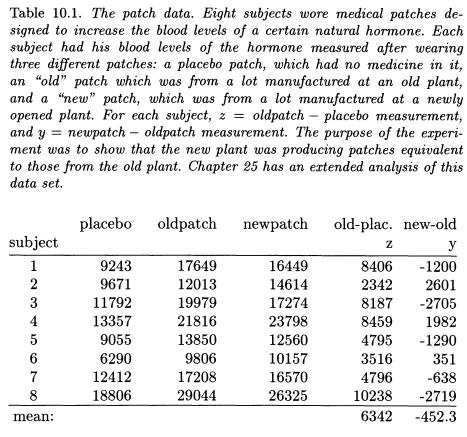
\includegraphics[width=\linewidth]{10/t10.1.png}
\newline

Целью эксперимента с пластырем было показать биоэквивалентность. Пластыри, изготовленные на старом заводе, уже были одобрены для продажи Управлением по санитарному надзору за качеством пищевых продуктов и медикаментов (FDA). Пластыри с нового завода не потребовали полного нового исследования FDA. Их одобрили бы к продаже, если бы можно было доказать, что они биоэквивалентны тем, что были изготовлены на старом заводе. Критерий биоэквивалентности FDA заключается в том, что ожидаемая эффективность новых пластырей соответствует ожидаемой эффективность старых пластырей в том смысле, что
\begin{equation}\label{eq10.5}
    \frac{\left|\mathrm{E}(\text{новый}) - \mathrm{E}(\text{старый})\right|}{\mathrm{E}(\text{старый}) - \mathrm{E}(\text{плацебо})} \leq 0.2.
\end{equation}
Другими словами, FDA хочет, чтобы новое лекарство соответствовало старому в пределах $20\%$ количества гормона, которое старый препарат добавляет к <<плацебо>> уровню крови.

Пусть $\theta$ параметр
\begin{equation}\label{eq10.6}
    \theta = \frac{\left|\mathrm{E}(\text{новый пластырь}) - \mathrm{E}(\text{старый пластырь})\right|}{\mathrm{E}(\text{старый пластырь}) - \mathrm{E}(\text{пластырь с плацебо})}.
\end{equation}
В главах 12--14 рассматриваются доверительные интервалы для $\theta$, подход, который приводит к полному ответу на вопрос о биоэквивалентности: <<действительно ли $|\theta| \leq 0.20$?.>>\footnote{В главе 25 представлен расширенный анализ биоэквивалентности этого набора данных.} Здесь мы рассматриваем только смещение и стандартную ошибку оценки метода подстановки $\hat{\theta}$.

Нас интересуют две статистики, $z_{i}$ и $y_{i}$, полученные для каждого из восьми субъектов,
\begin{equation}\label{eq10.7}
   z = \text{измерение при старом пластыре} - \text{измерение при плацебо}
\end{equation}
и
\begin{equation}\label{eq10.8}
   y = \text{измерение при новом пластыре} - \text{измерение при старом пластыре}.
\end{equation}

Предполагая, что пары $x_{i} = (z_{i}, y_{i})$ получены путем случайной выборки из неизвестного двумерного распределения $F$, $F \rightarrow x = (x_{1}, x_{2} \dots x_{8})$, тогда $\theta$ в (\ref{eq10.6}) это параметр
\begin{equation}\label{eq10.9}
   \theta = t(F) = \frac{E_{F}(y)}{E_{F}(z)}.
\end{equation}

В этом случае $t(\cdot)$ является функцией, которая принимает распределение вероятностей $F$ на парах $x = (z, y)$ и выдает отношение математических ожиданий. Оценка метода подстановки $\theta$ равна
\begin{equation}\label{eq10.10}
   \hat{\theta} = t(\hat{F}) = \frac{\Bar{y}}{\Bar{z}} = \frac{\sum_{i=1}^{8}y_{i}/8}{\sum_{i=1}^{8}z_{i}/8},
\end{equation}
которую мы возьмем за нашу оценку $\hat{\theta} = s(X)$. Обратите внимание, что ничто в этих формулировках не предполагает, что $z$ и $y$ независимы друг от друга. Последние два столбца таблицы 10.1 показывают $z_{i}$ и $y_{i}$ для восьми испытуемых. Значение $\hat{\theta}$ равно
\begin{equation}\label{eq10.11}
   \hat{\theta} = \frac{-452.3}{6342} = -0.0713.
\end{equation}
Мы видим, что $|\hat{\theta}|$ значительно меньше $0.2$, так что есть некоторая надежда на выполнение условия биоэквивалентности FDA.

На рисунке 10.1 показана гистограмма $B = 400$ бутстреп репликаций $\hat{\theta}$, полученных как в (6.1--6.2): бутстреп выборки $x^{*} = (x_{1}^{*}, x_{2}^{*}, \dots, x_{8}^{*}) =\\=(x_{i_1}, x_{i_2}, \dots, x_{i_8})$ дают бутстреп репликации
\begin{equation}\label{eq10.12}
   \hat{\theta}^{*} = \frac{\Bar{y}^{*}}{\Bar{z}^{*}} = \frac{\sum_{j=1}^{8}y_{i_j}/8}{\sum_{j=1}^{8}z_{i_j}/8}.
\end{equation}

\noindent
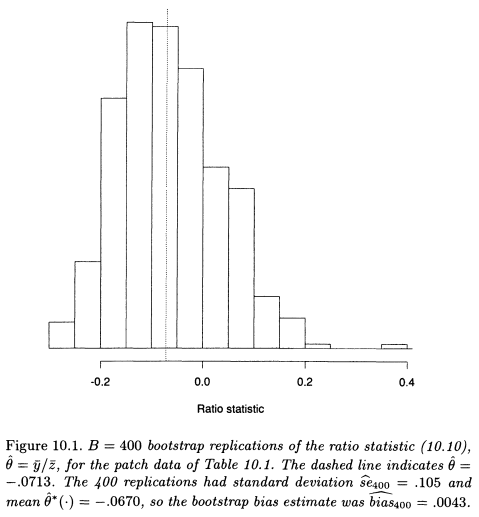
\includegraphics[width=\linewidth]{10/f10.1.png}
\newline

Для $400$ репликаций стандартное отклонение выборки составило $\widehat{se}_{400} = 0.105$, а среднее значение выборки $\hat{\theta}^{*}(\cdot) = -0.0670$. Бутстреп оценка смещения составляет
\begin{equation}\label{eq10.12}
   \widehat{\text{bias}}_{400} = -0.0670 - (-0.0713) = 0.0043.
\end{equation}
Это вычисление основано на формуле (\ref{eq10.4}), с использованием того факта, что в данном случае $\hat{\theta} = t(\hat{F})$.

Отношение оцененного смещения к стандартной ошибке $\widehat{\text{bias}}_{400}/\widehat{\text{se}}_{400} = 0.041$ мало, что указывает на то, что в этом случае нам не нужно беспокоиться о смещении $\hat{\theta}$. Как правило, смещение меньшее чем $0.25$ стандартных ошибок можно игнорировать, если мы не пытаемся провести аккуратные вычисления доверительных интервалов. Среднеквадратичная ошибка оценки $\hat{\theta}$ для $\theta$ есть $$\sqrt{\mathrm{E}_{F}\left[(\hat{\theta} - \theta)^{2}\right]}$$ мера точности, которая учитывает как смещение, так и стандартную ошибку. Можно показать, что значение среднеквадратичной ошибки равно
\begin{equation*}
   \sqrt{\mathrm{E}_{F}\left[(\hat{\theta} - \theta)^{2}\right]} = \sqrt{\text{se}_{F}(\hat{\theta})^{2} + \text{bias}_{F}(\hat{\theta}, \theta)^{2}} =
\end{equation*}
\begin{equation}\label{eq10.14}
   =\text{se}_{F}(\hat{\theta}) \cdot \sqrt{1 + \left(\frac{\text{bias}_{F}}{\text{se}_{F}}\right)^{2}} \doteq \text{se}_{F}(\hat{\theta}) \cdot \left[1 + \left(\frac{\text{bias}_{F}}{\text{se}_{F}}\right)^{2}\right].
\end{equation}
Если $\text{bias}_{F} = 0$, то среднеквадратичная ошибка равна её минимальному значению $\text{se}_{F}$. Если $|\text{bias}_{F}/\text{se}_{F}| < 0.25$, тогда среднеквадратичная ошибка не превосходит $\text{se}_{F}$ больше, чем примерно на $3.1\%$.

Мы знаем, что $B = 400$ бутстреп репликаций обычно более чем достаточно для получения хорошей оценки стандартной ошибки. Достаточно ли этого, чтобы получить хорошую оценку смещения? Ответ в данном конкретном случае --- нет. Помните, что в определении идеальной бутстреп оценки смещения  $\widehat{\text{bias}}_{\infty} = \text{bias}_{\hat{F}}$ (\ref{eq10.2}),  $\widehat{\text{bias}}_{B}$ (\ref{eq10.4}) заменяет $E_{\hat{F}}(\hat{\theta}^{*})$ на $\hat{\theta}^{*}(\cdot)$. По распределению бутстреп репликаций мы можем сказать, насколько хорошо $\hat{\theta}^{*}(\cdot)$ оценивает $\mathrm{E}_{\hat{F}}(\hat{\theta}^{*})$. Применение (5.6) дает
\begin{equation}\label{eq10.15}
    \text{Prob}_{\hat{F}}\left\{\left|\hat{\theta}^{*}(\cdot)-\mathrm{E}_{\hat{F}}\{\hat{\theta}^{*}\}\right| < 2\frac{\widehat{\text{se}}_{B}}{\sqrt{B}}\right\}
    = \text{Prob}_{\hat{F}}\left\{\left|\widehat{\text{bias}}_{B}-\widehat{\text{bias}}_{\infty}\right| < 2\frac{\widehat{\text{se}}_{B}}{\sqrt{B}}\right\} \doteq 0.95,
\end{equation}
где $\widehat{\text{se}}_{B}$ --- бутстреп оценка стандартной ошибки. Для бутстреп данных на рисунке 10.1 с $\widehat{\text{se}}_{B} = 0.105$ и $B = 400$, мы получаем
\begin{equation}\label{eq10.16}
    \text{Prob}_{\hat{F}}\left\{\left|\widehat{\text{bias}}_{B}-\widehat{\text{bias}}_{\infty}\right| < 0.0105\right\} \doteq 0.95,
\end{equation}
большой диапазон погрешности по сравнению с расcчитанным значением $\widehat{\text{bias}}_{400} = 0.0043$.

Граница ошибки $0.0105$ в (\ref{eq10.16}) достаточно мала, чтобы показать, что смещение здесь не является большой проблемой: так как $\widehat{\text{bias}}_{400} = 0.0043$, мы, вероятно, имеем $|\widehat{\text{bias}}_{\infty}| < 0.0043 + 0.0105 = 0.0148$ и поэтому $|\widehat{\text{bias}}|/\widehat{\text{se}} < 0.0148 / 0.106 = 0.14$. Что довольно меньше, чем эмпирическое граница $0.25$. Однако нам все еще может быть интересно узнать $\widehat{\text{bias}}_{\infty}$ или хорошее приближение к нему и вычислениям (\ref{eq10.16}), показывающим что $\widehat{\text{bias}}_{400} = 0.0043$, нельзя доверять. Мы могли бы просто увеличить $B$, но в этом нет необходимости.